\part{Theorie}
\cref{fig:Einleitung/SchaltbildOperationsverstärker} zeigt das Schaltsymbol, 
welches für einen beliebigen Operationsverstärker gilt. Dieser hat einen 
"`Plus"'-Eingang ($+$) und einen "`Minus"'-Eingang ($-$) und einen Ausgang A.

\begin{figure}[H]
	\centering
	\begin{subfigure}[t]{0.3\linewidth}
		\centering
		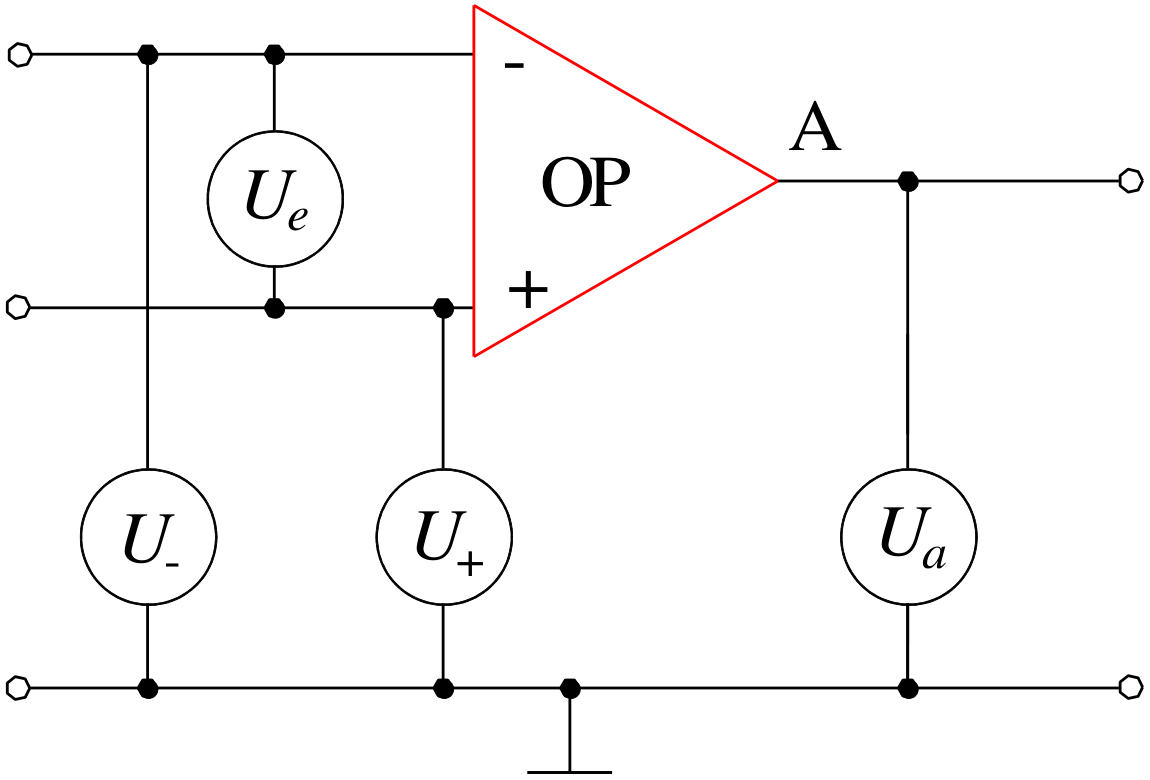
\includegraphics[width=\linewidth]{theorie/schaltbildOP}
		\caption{Schaltbild eines Operationsverstärkers ({\color{red} rot}), 
		entnommen aus \cite{script}}
		\label{fig:Einleitung/SchaltbildOperationsverstärker}
	\end{subfigure}
	\quad
	\begin{subfigure}[t]{0.2\linewidth}
		\centering
		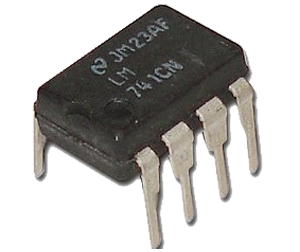
\includegraphics[width=\linewidth]{theorie/741}
		\caption{Abbild eines Operationsverstärkers vom Typ 741, entnommen aus 
		\cite{image741}}
		\label{fig:Einleitung/Operationsverstärker}
	\end{subfigure}
	\quad
	\begin{subfigure}[t]{0.3\linewidth}
		\centering
		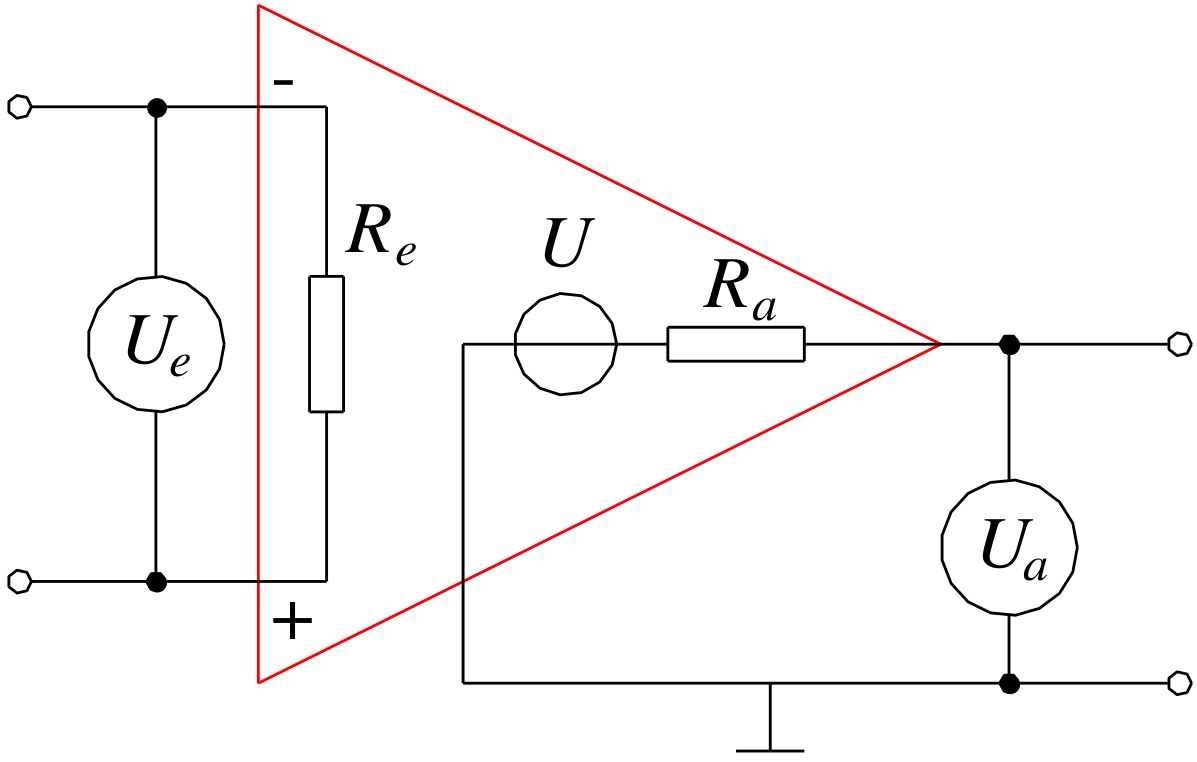
\includegraphics[width=\linewidth]{theorie/ersatzSchaltbildOP}
		\caption{Ersatzschaltbild eines Operationsverstärkers ({\color{red} 
		rot}) zur Definition es Eingangswiderstandes $R_e$ und des 
		Ausgangswiderstandes $R_a$, entnommen aus \cite{script}}
		\label{fig:Einleitung/ErsatzschaltbildOperationsverstärker}
	\end{subfigure}
	\caption{Darstellungen eines Operationsverstärkers}
\end{figure}

Der Operationsverstärker verstärkt hierbei die 
\textsl{Eingangsspannungsdifferenz} $U_e$:
\begin{equation}\label{eq:Eingangsspannungsdifferenz}
	U_e = U_+ - U_-
\end{equation}
mit dem \textsl{Leerlaufverstärkungsfaktor} $V_0 > 0$, womit für die 
\textsl{Ausgangsspannung} $U_a$ gilt:
\begin{equation}\label{eq:Ausgangsspannung}
	U_a = V_0 \cdot U_e = V_0 \cdot \left(U_e = U_+ - U_-\right).
\end{equation}
Wenn $U_- = \qty{0}{\V}$ folgt aus \cref{eq:Ausgangsspannung}:
\begin{equation}
	U_- = \qty{0}{\V} \quad \rightarrow \quad U_a = V_0 \cdot U_+
\end{equation}
In diesem Fall haben sowohl die Eingangs- als auch die Ausgangsspannung das 
gleiche Vorzeichen. Daher wird der "`Plus"'-Eingang als 
\textsl{nicht-invertierender} Eingang bezeichnet. Im Gegensatz dazu gilt für 
den Fall
\begin{equation}
	U_+ = \qty{0}{\V} \quad \rightarrow \quad U_a = -V_0 \cdot U_-
\end{equation}
dass die Eingangsspannung $U_-$ und die Ausgangsspannung $U_a$ entgegengesetzte 
Vorzeichen haben. Daher wird der "`Minus"'-Eingang eines Operationsverstärkers 
auch \textsl{invertierender} Eingang genannt.

Ein idealer Operationsverstärker hat einen unendlich großen 
Leerlaufverstärkungsfaktor $V_0 \rightarrow \infty$ (vgl. 
\cref{fig:Einleitung/ErsatzschaltbildOperationsverstärker}), einen unendlich 
großen 
Eingangswiderstand $R_e \rightarrow \infty$ (vgl. 
\cref{fig:Einleitung/ErsatzschaltbildOperationsverstärker}), einen 
verschwindend kleinen Ausgangswiderstand $R_a \rightarrow 0$ (vgl. 
\cref{fig:Einleitung/ErsatzschaltbildOperationsverstärker}) und eine 
frequenzunabhängige Verstärkung. Ein realer Operationsverstärker weicht 
natürlich von diesem Idealvorstellungen ab: die Widerstände sind weder 
unendlich groß noch verschwindend klein, auch der Leerlaufverstärkungsfaktor 
hat seine Grenze und die Verstärkung findet frequenzabhängig statt.

Für die folgenden Überlegungen wird jedoch trotzdem der Operationsverstärker 
als eine "`Black Box"' angenommen und mit den idealen Eigenschaften betrachtet.

\section{Mit- und Gegenkopplung}
Aufgrund des großen Leerlaufverstärkungsfaktors $V_0$ ist der 
Operationsverstärker nicht ohne äußere Beschaltung nutzbar, da nach
\cref{eq:Ausgangsspannung} bereits kleine Eingangsspannungsdifferenzen $U_e$ im
\unit{\micro\V}- bis \unit{\mV}-Bereich zum Erreichen der maximalen 
Ausgangsspannung führen. Die maximale Ausgangsspannung ist hierbei abhängig von
der eingesetzten Betriebsspannung, welche typischerweise $\pm \qty{12}{\V}$
beträgt. Aufgrund dieses Verhaltens wird ein teil der Ausgangsspannung
auf den invertierenden Eingang des Operationsverstärkers zurückgekoppelt. Dies
hat zur Folge, dass eine Änderung der Ausgangsspannung einer Änderung der
Eingangsspannungsdifferenz $U_e$ entgegenwirkt. Daher auch der Name 
"`Gegenkopplung"'

Würde nun umgekehrt eine Änderung der Ausgangsspannung auch eine gleichsinnige
Änderung des Eingangsspannungsdifferenz bewirken, da ein Teil der 
Ausgangsspannung auf den nicht-invertierenden Eingang zurückgekoppelt wird, so
wäre der Operationsverstärker Mitgekoppelt und der Operationsverstärker Würde
übersteuern.

In den folgenden Abschnitten werden verschiedene Schaltungen eines 
Operationsverstärkers betrachtet.

\section{Beschaltungen eines Operationsverstärkers}
\subsection{Invertierender Verstärker}
Für einen invertierenden Verstärker wird eine gegengekoppelte Beschaltung des
Operationsverstärkers gemäß \cref{fig:Theorie/invertierenderVerstärker} 
betrachtet.

\begin{figure}[H]
	\centering
	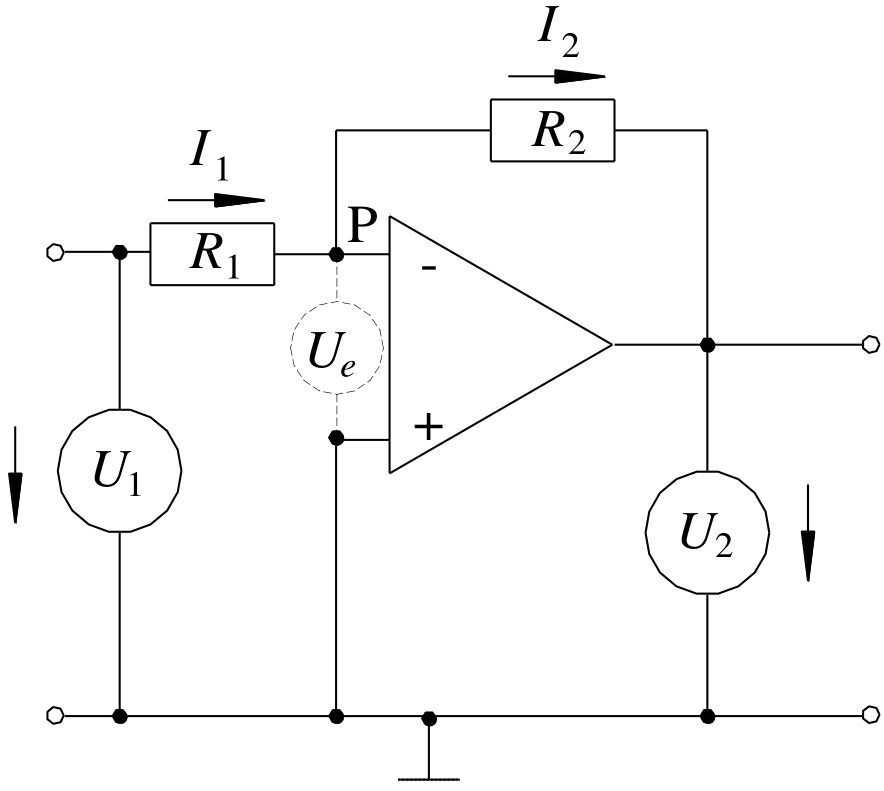
\includegraphics[width=0.3\linewidth]{theorie/schaltbild-invertierenderVerstärker}
	\caption{Invertierender Verstärker. Alle Spannungen werden auf das 
	Massepotential bezogen. Die Klemmenspannung $U_1$ zwischen den 
	Eingangsbuchsen (offene Kreise links) angelegt. Die Ausgangsspannung wird
	ziwschen den Ausgangsbuchsen (offene Kreise rechts) abgegriffen, entommen
	aus \cite{script}}
	\label{fig:Theorie/invertierenderVerstärker}
\end{figure}

Die zu verstärkende Klemmenspannung $U_1$ wird über den Widerstand $R_1$ auf den
invertierenden Eingang des Operationsverstärkers gegeben, auf den gleichzeitig
über den Widerstand $R_2$ die Ausgangsspannung $U_2$ zurückgekoppelt wird.

Aufgrund des hohen Eingangswiderstandes es Operationsverstärkers fließt
praktisch kein Strom in den Operationsverstärker. Somit gilt nach der 
Knotenregel für den Punkt P:
\begin{equation}
	I_1 - I_2 = 0
\end{equation}
woraus folgt, dass:
\begin{equation}
	I_1 = I_2 := I
\end{equation}
